\documentclass{article}
\usepackage[utf8]{inputenc}
\usepackage{wasysym}
\usepackage{qrcode}
\usepackage[colorlinks]{hyperref}
\usepackage{lmodern}
\usepackage{graphicx}
\usepackage{xcolor}
\usepackage[left=2cm, top=3cm, right=2cm]{geometry}
\usepackage{minted}
\usepackage{svg}
\usepackage{xcolor}
\definecolor{LightGray}{gray}{0.975}

%setup new colors
\hypersetup{
%linkcolor=blue
%,citecolor=
%,filecolor=
urlcolor=blue
%,menucolor=
%,runcolor=
%,linkbordercolor=
%,citebordercolor=
%,filebordercolor=
%,urlbordercolor=
%,menubordercolor=
%,runbordercolor=
}

\title{Database Administration \\ Lab 02: Reverse Design}
\author{Andrés Oswaldo Calderón Romero, Ph.D.}
\date{\today}

\begin{document}

\maketitle

\section{Introduction}
The main objective of this lab is to explore a database tool to work on the DBA database design, specifically with the technique of Reverse Design to obtain an ERD. \href{https://dbeaver.io/}{DBeaver} is a multiplatform DBA tool designed for diverse DBMSs. It is a Java-based application with a GUI that can connect to a database (via a JDBC driver), extract the required data, and generate an ERD from scratch. We will cover a basic guide using a couple of DBMSs, complete some sections of the online course, and then explore other online alternatives as independent work.


\section{DBeaver Tutorial}
\subsection{Installation}
We will follow the steps for installing DBeaver on Linux because we will need PostgreSQL later on. We assume that you have already a running install of PostgreSQL running on your system (via Vagrant or Docker), but this is not a strict requirement. You can install DBeaver on Windows or macOS, but we will assume that you have a rolling installation of PostgreSQL on your machine.

That said, you can download the DBeaver installer from the Download section at \url{https://dbeaver.io/download/}. In the case of Linux, we will download the \href{https://dbeaver.io/files/dbeaver-ce-latest-linux.gtk.x86_64.tar.gz}{Linux (tar.gz)} option.  You should follows the appropiate instruction if decide to work in other O.S.

You only need to uncompress the file, and you are ready to go! So let's follow these steps:

\begin{enumerate}
    \item Open a terminal console and type:
    \begin{minted}
    [tabsize=4, obeytabs, frame=lines, framesep=2mm, baselinestretch=1.2, bgcolor=LightGray, fontsize=\footnotesize]{bash}
    wget https://dbeaver.io/files/dbeaver-ce-latest-linux.gtk.x86_64.tar.gz
    \end{minted}

    \item Decompress the tar file by executing:
    \begin{minted}
    [tabsize=4, obeytabs, frame=lines, framesep=2mm, baselinestretch=1.2, bgcolor=LightGray, fontsize=\footnotesize]{bash}
    tar -zxvf dbeaver-ce-latest-linux.gtk.x86_64.tar.gz
    \end{minted}

    \item Now, you can execute DBeaver from your terminal by navigating inside the dbeaver folder and running the executable. Type the following commands:
    \begin{minted}
    [tabsize=4, obeytabs, frame=lines, framesep=2mm, baselinestretch=1.2, bgcolor=LightGray, fontsize=\footnotesize]{bash}
    cd dbeaver
    ./dbeaver
    \end{minted}
\end{enumerate}

If everything goes well, you will see something like Figure \ref{fig:dbeaver}.

\begin{figure}[t]
    \centering
    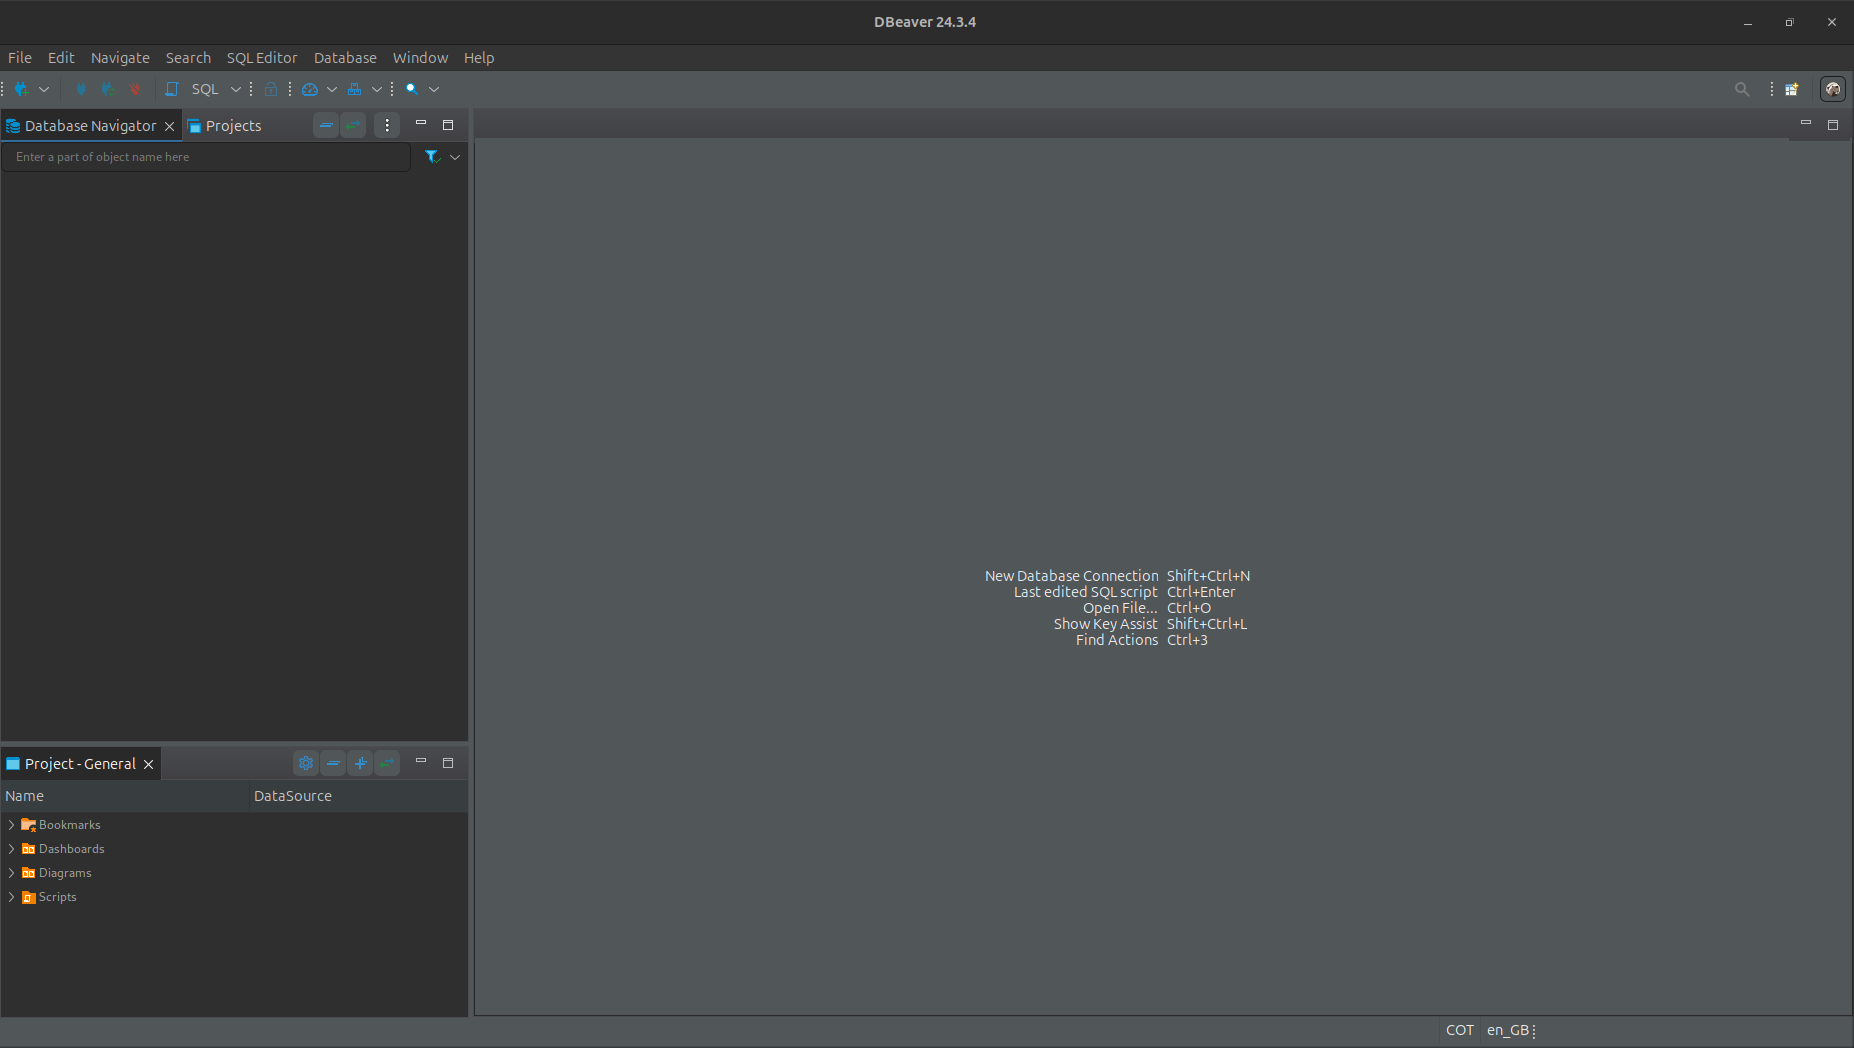
\includegraphics[width=\textwidth]{figures/dbeaver}
    \caption{DBeaver GUI.}
    \label{fig:dbeaver}
\end{figure}

\subsection{Reverse ERD using SQLite}
Overall, this will be very simple. We will connect to a sample database called Chinook, implemented in \href{https://www.sqlite.org/}{SQLite3}. SQLite is a highly portable DBMS, and you will not need any additional installation (I believe?). You can download the database from \href{https://drive.google.com/file/d/1BWhCaN7Bp989HNRn55sO7lB7k-9aBwbS/view?usp=sharing}{here}.

Follow this \href{https://drive.google.com/file/d/1d04-Wx6gUBqxyDga-DLC4kZKiKGjq62F/view?usp=sharing}{video} to explore the steps for generating the ERD for this database by making the connection from DBeaver. Let's go!

\subsection{Reverse ERD using PostgreSQL}
Ok, now we will give our PostgreSQL installation a try with an interesting sample database named \href{https://github.com/devrimgunduz/pagila}{Pagila}. You can download the database schema from \href{https://drive.google.com/file/d/1XAHXlBIfAxmSvh8bWeMIy81YppZXu21w/view?usp=sharing}{here} and the actual data from \href{https://drive.google.com/file/d/1l3_LFHdKv9YvfaQ-aZoqeDMOjSkLTmqR/view?usp=sharing}{here}.

Again, follow this new \href{https://drive.google.com/file/d/1394GbIGQkrgSWgQN9jtLSjVkbp7NC226/view?usp=sharing}{video} to explore the steps for generating the ERD, this time by connecting to a PostgreSQL instance. Here we go!

\section{Independent Work}
\subsection{Complete Others Sections in the Course}
You are asked to create an account on Udemy and visit the webpage of the \href{https://www.udemy.com/course/database-design-and-management/}{\textit{Database Design and Management}} course. Follow sections 2 and 4. Once you complete those sections, please take a screenshot of your progress (see Figure \ref{fig:progress} for an example) and attach it to your report.

\begin{figure}[t]
    \centering
    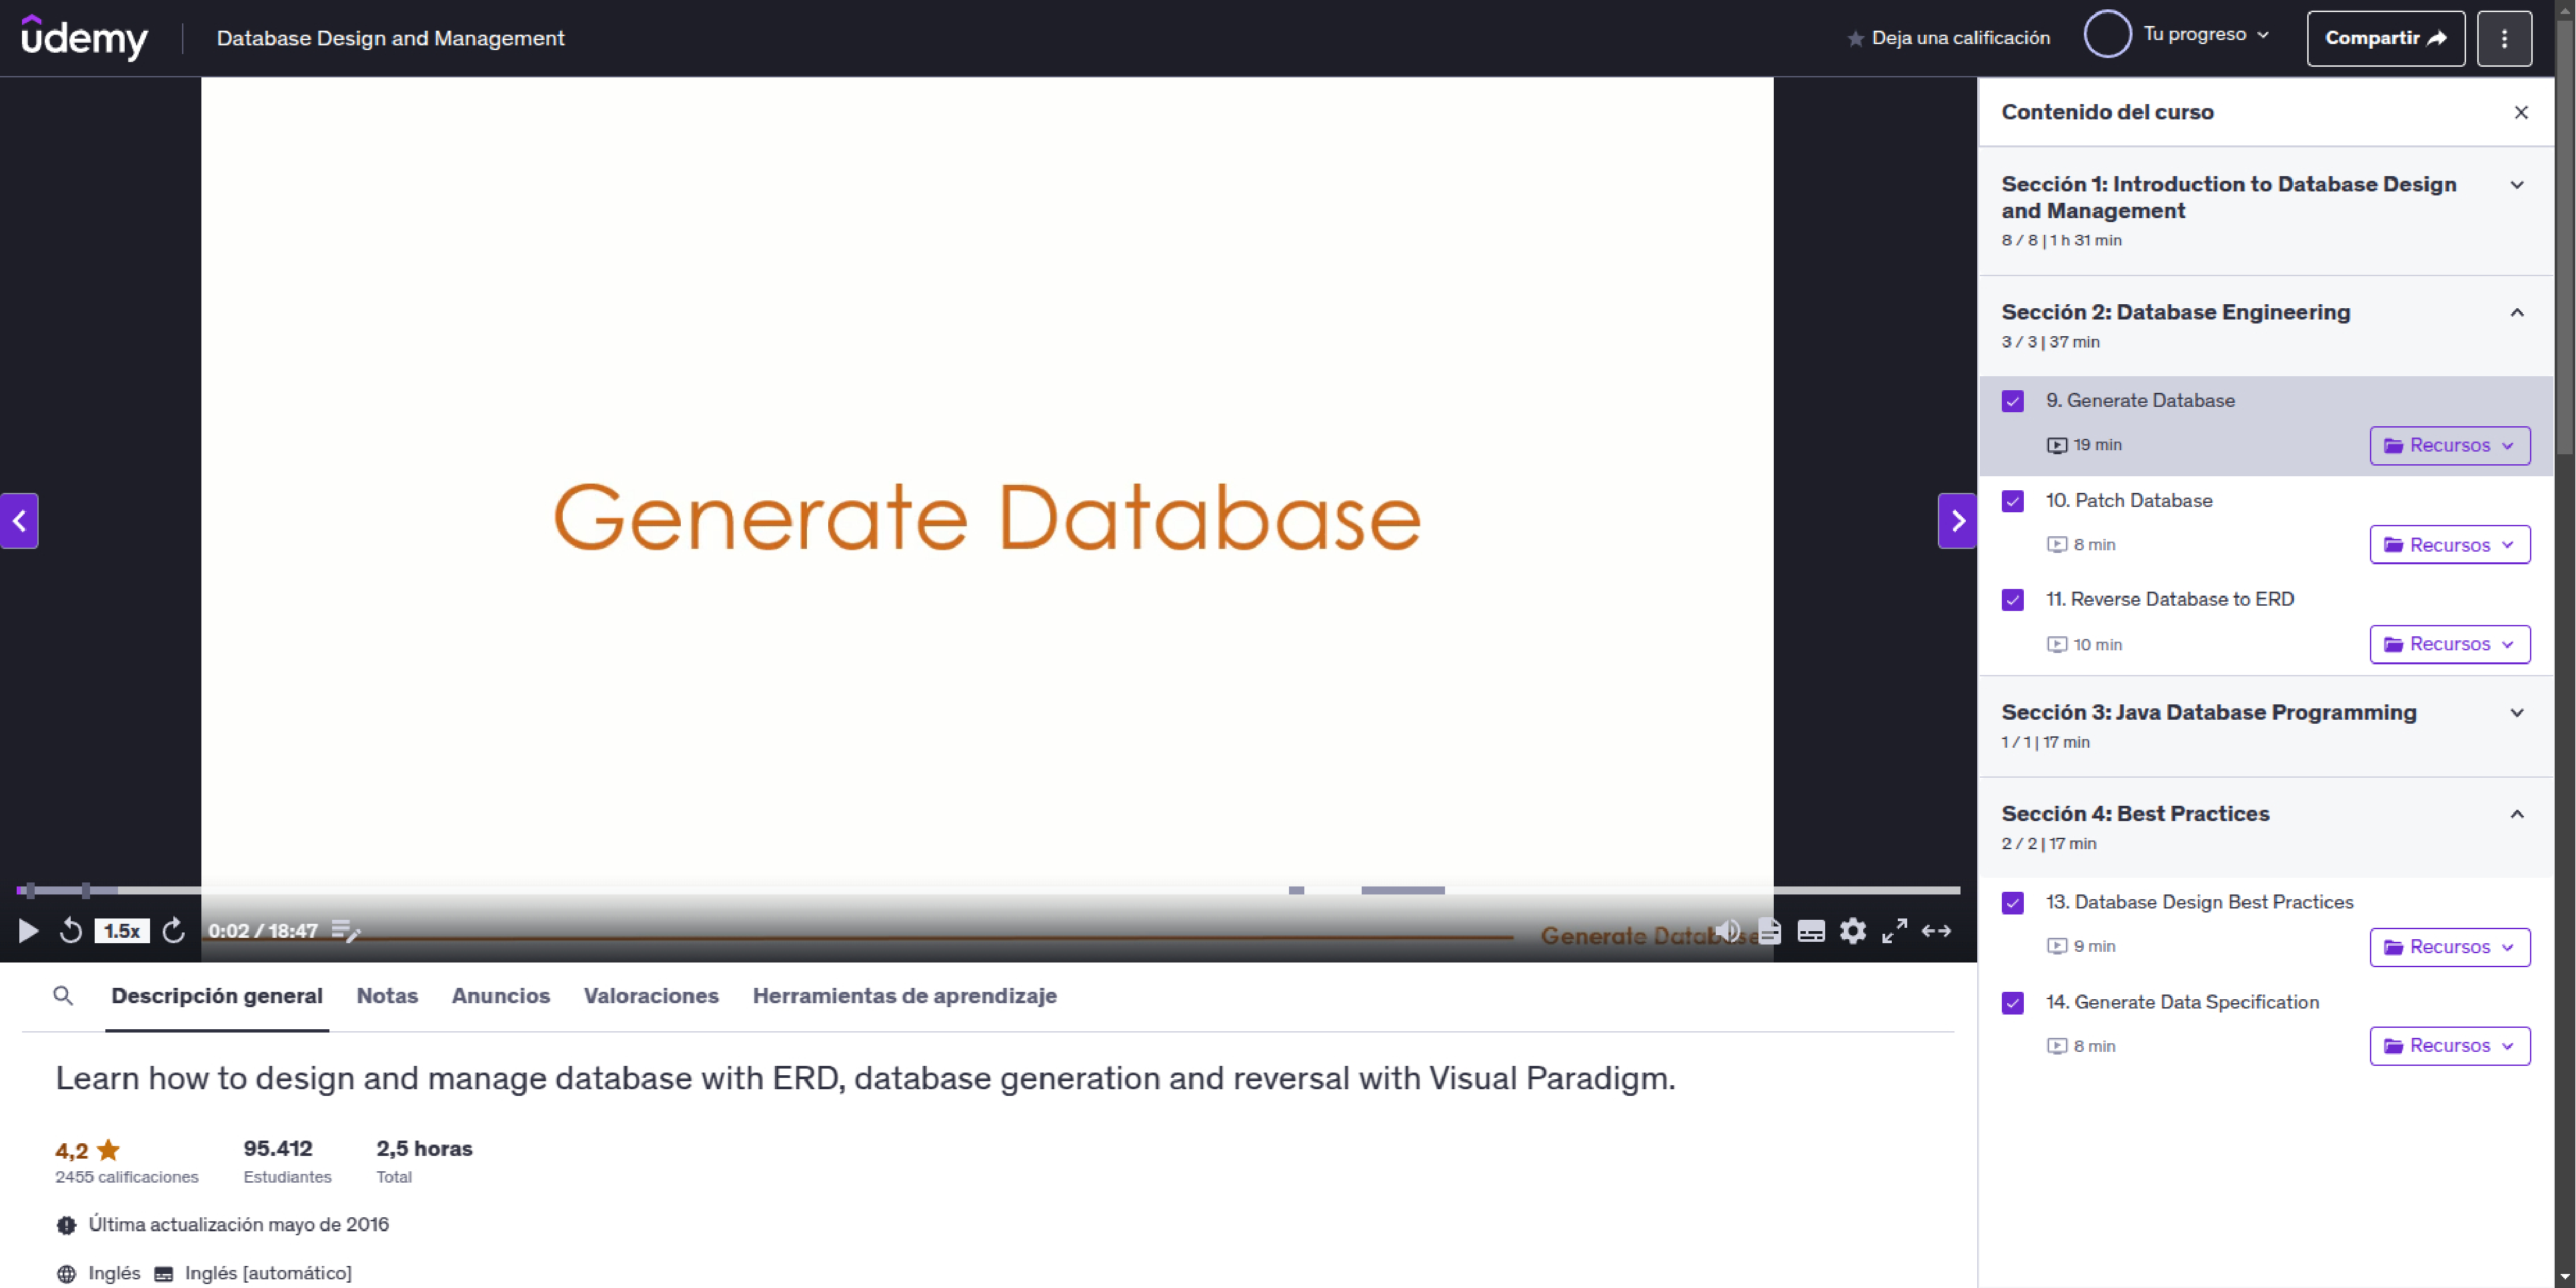
\includegraphics[width=0.75\textwidth]{figures/progress}
    \caption{Progress in the \textit{Database Design and Management} Udemy course (checkboxes on the right).}
    \label{fig:progress}
\end{figure}

\subsection{Explore Others Options}
As before, we will now explore the same topic using a similar approach but this time by trying out online tools for creating E-R diagrams. Read the list of a few interesting tools \href{https://drive.google.com/file/d/1FEkgTJEXY07AtVxIYr1_qq0naw3rmOpu/view?usp=sharing}{here}.

So, you will have a list of E-R Diagram tools:

\begin{itemize}
    \item Azimutt
    \item draw.io
    \item Lucidchart
    \item QuickDBD
    \item DBDiagram.io
    \item DrawSQL
    \item Dia
\end{itemize}

and a list of DBMSs:

\begin{itemize}
    \item Oracle
    \item SQLServer
    \item MySQL
    \item DB2
\end{itemize}

Now you will choose a combination of a E-R Diagram tool and a DBMS (i.e. Lucidchart + MySQL) and then write a well-structured tutorial on how to use that tool to generate or create ERDs for the \textbf{Chinook} database for that particular DBMS.

We expect you to submit your report by \textbf{August 18, 2025}, via the link that will be provided on Brightspace.

\vspace{5mm}
Happy Hacking \includesvg[width=4mm]{figures/sunglasses}!

\end{document}

